\section{Main Part}\label{sec:main}

Listing~\ref{lst:example}.
See \figurename~\ref{fig:example1} and
%\figurename~\ref{fig:example2}.

Also \tablename~\ref{tbl:table1}.
% and \equationname~\ref{eq:var_idb}.

\lstset{language=Java, caption=Example Code, label=lst:example}
\lstinputlisting{resources/code/example.java}

\small
\begin{equation}
  \begin{array}{l}
    \displaystyle t^{p_d}_{fw}(d) = max_{d}(t_{child_{i}}) \\
    \displaystyle t^{p_d}_{db}(d) = \sum_{i=1}^{d} t_{db_{i}} \\
    \displaystyle t^{p_d}_{pc}(n,d) =
    	\begin{cases}
        	t_{pc}(d) + c(n) & \text{if $d = 1$,}\\
        	t_{pc}(d) + c(n) + max(t_{avail}(d)) & \text{if $d>1$.}\\
        \end{cases}
  \end{array}
  \label{eq:var_idb}
\end{equation}
\normalsize

\begin{figure}
    \centering
    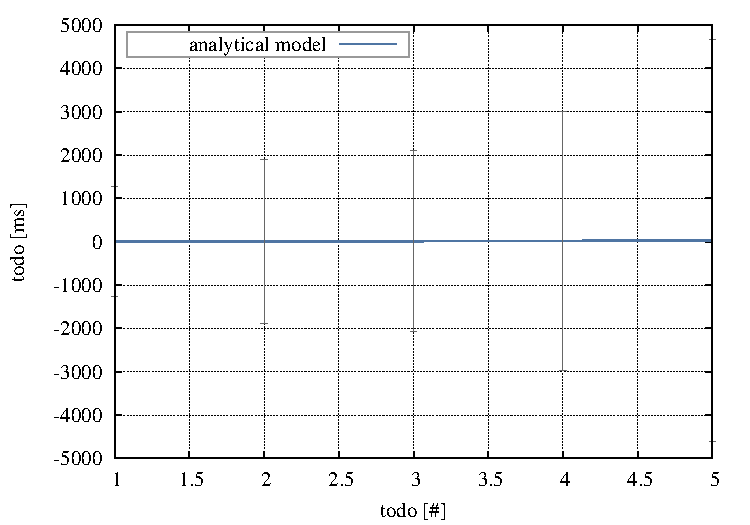
\includegraphics[width=.45\textwidth]{resources/images/example1.pdf} 
    \caption{Example image.}
    \label{fig:example1}
\end{figure}

\begin{figure}
    \centering
    \subfloat[example2]{
        \label{fig:example2}
        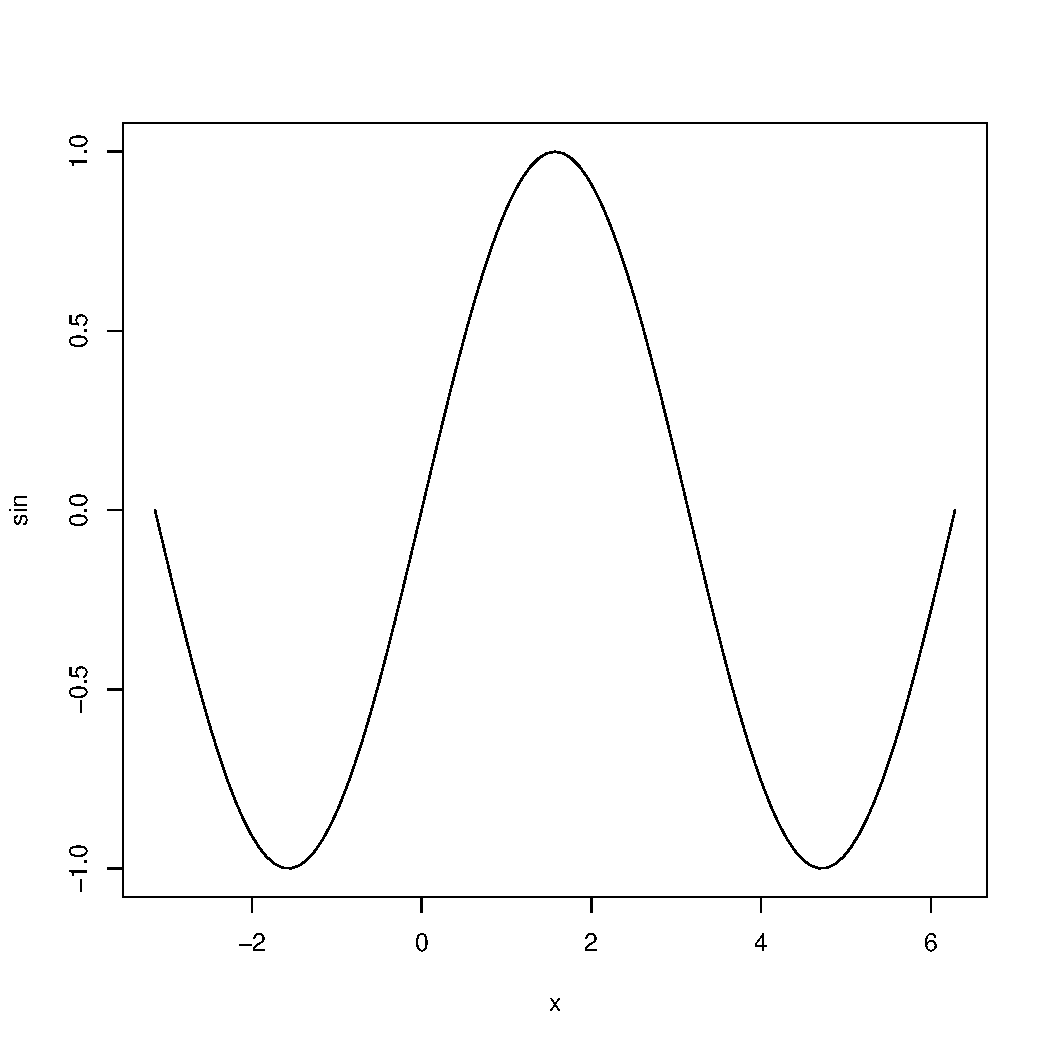
\includegraphics[width=.2\textwidth]{resources/images/example2.pdf}
    }
    \subfloat[example3]{
        \label{fig:example3}
        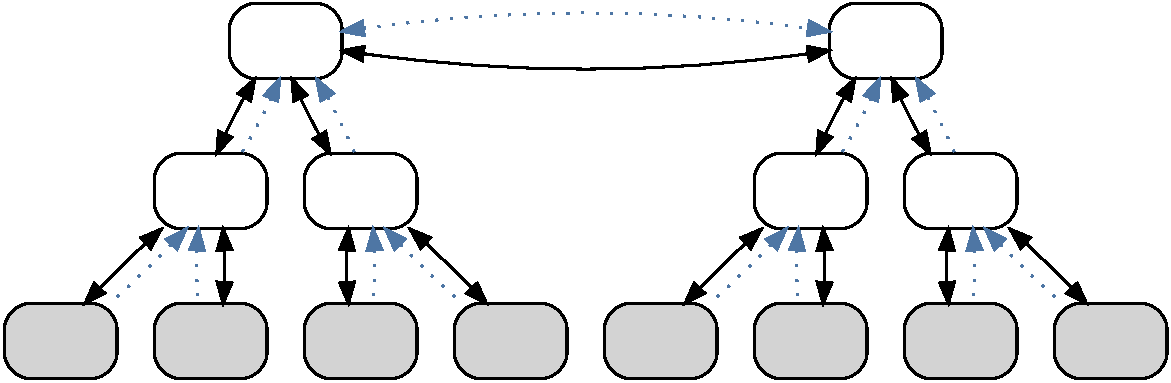
\includegraphics[width=.2\textwidth]{resources/images/example3.pdf} 
    }
    \caption{Example images.}
    \label{fig:exammple2_3}
\end{figure}

\begin{table}
    \centering
    \caption{Example table.}
    \begin{tabular}{ll}\toprule
    \textbf{Name}  & \textbf{Age} \\ \midrule
    Hans           & 80             \\
    Heinrich       & 77             \\
    Herbert        & 84             \\ \bottomrule
    \end{tabular}
    \label{tbl:table1}
\end{table}

